\documentclass{beamer}
\usepackage{hyperref}
\usepackage{xcolor}
\usepackage{graphicx}
% Theme choice:
\usetheme{CambridgeUS}

% Title page details: 
\title{Modelo predictivo del crecimiento urbano} 
\subtitle{Equipo \#2}
\author{\textit{Estimación de la capacidad de carga poblacional}}
\date{\today}
\logo{\large \LaTeX{}}

\begin{document}

% Title page frame

\begin{frame}
    \titlepage 
    \underline{\textbf{Integrantes: }}\\
    Luis Ernesto Serras Rimada \\ Guillermo Cepero García \\ Miguel Vadim Vilariño Pedraza
\end{frame}

% Remove logo from the next slides
\logo{}
\author{\textit{\underline{\textbf{Equipo \#2}}}}

\section{Introducción}
\begin{frame}{Modelo de crecimiento urbano}
    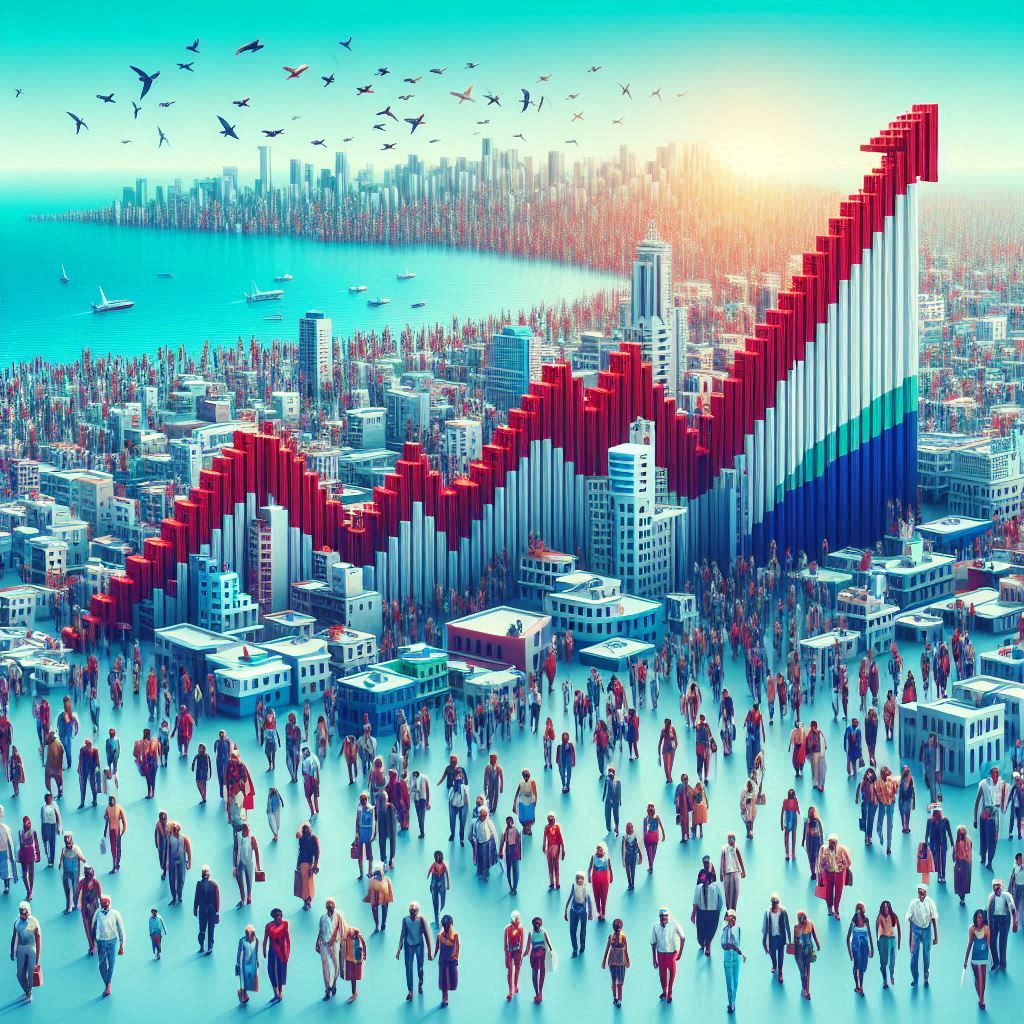
\includegraphics[height = 7cm]{img/cuba1.jpeg}
\end{frame} 

\section{Desarrollo}
\begin{frame}

\textit{Entonces se tiene que:}
\begin{itemize}
    \item (P(t)) es la población en función del tiempo (t).
    \item (r) es la tasa de crecimiento intrínseca de la población.
    \item (K) es la capacidad de carga o tamaño máximo sostenible de la población.
\end{itemize}\\

\textit{\underline{Parámetros a Estimar:}}
\begin{itemize}
    \item (r): Tasa de crecimiento intrínseca de la población. 
    \item (K): Capacidad de carga de la población.
\end{itemize}
\end{frame}

\section{Ecuación Diferencial}
\begin{frame}{Modelo logístico}
$$\frac{dP}{dt} = r \cdot P(t)(1 - \frac{P(t)}{K}) $$

\underline{Para la tasa de crecimiento intrinseca se tiene que:} $$r = (\frac{N(t)-F(t)}{P(t)})$$
\end{frame}

\subsection{Modelo Matemático}
\begin{frame}{Modelo Matemático}
    \underline{La función logística tiene la forma:} $$P(t) = \frac{K}{1 + Ae^{-rt}}$$
    \underline{La ecuación para encontrar (A) es:} $$P(0) = \frac{K}{1 + Ae^{0}}$$
\end{frame}

\subsection{Modelo Numérico}
\begin{frame}{curvefit}
    Minimizar: $\sum_{i=1}^{N} (y_{i} - f(x_{i}, \theta))^2 $ 
Donde:\\
\begin{itemize}
	\item $y_{i}$ son los valores medidos
	\item $x_{i}$ son los valores independientes
	\item f($x_{i}, \theta$) es la función modelo con parámetros θ
	\item	$\sum$ denota la suma sobre todos los puntos de datos
\end{itemize}
\end{frame}

\begin{frame}{curve-fit}
    \textbf{Definición inicial:} Se proporciona una función modelo f($x, \theta$) y los datos experimentales (xdata, ydata).\\
    \textbf{Inicialización:} Se establecen valores iniciales para los parámetros $\theta$.\\
    \textbf{Cálculo de residuales:} Se calcula la diferencia entre los datos mediantes y la función modelo:\\ r = ydata - f($xdata, \theta$)\\
    \textbf{Derivación:} Se calcula la derivada de los residuales respecto a cada parámetro:\\
    $$	\frac{\partial_{r}}{\partial \theta_{j}} = -\frac{\partial_{f}}{\partial \theta_{j}} $$
\end{frame}

\begin{frame}{curve-fit}
    \textbf{Iteración:} Se actualiza cada parámetro $\theta_{j}$ según la fórmula de Levenberg-Marquardt:\\
    $$\theta_{j}^{(n+1)} = \theta_{j}^{n} - [J^{T} J]^{-1} J^{T} r $$

    Donde J es la matriz Jacobiana: $$\frac{\partial_{r}}{\partial \theta_{j}}$$
    \textbf{Convergencia:} El proceso se repite hasta que se alcance un criterio de convergencia.\\ \\
    \underline{\large{\textbf{Adaptación al modelo logístico: }}}\\
    La función curvefit intentará minimizar la suma de los cuadrados de los residuales para encontrar los valores óptimos de $K$ y $r$ que minimizan esta expresión. 
\end{frame}
% Blocks frame
\section{Resultados}
\begin{frame}{Modelo sin intervalos}
    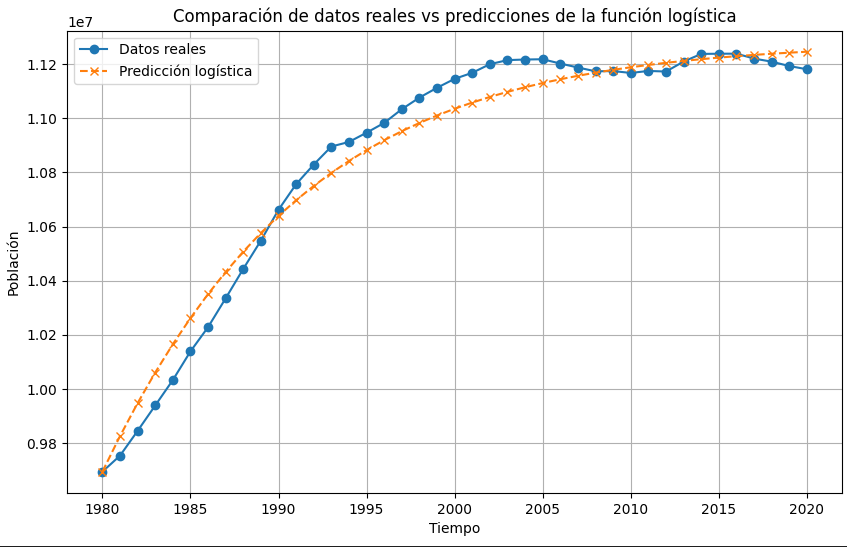
\includegraphics[height = 7cm]{img/graph_img/reales_vs_logistic.png}
\end{frame} 

\begin{frame}{DataFrame para intervalos de 5 años}
    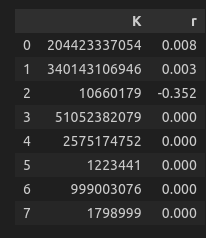
\includegraphics[height = 7cm]{img/graph_img/df5.png}
\end{frame} 


\begin{frame}{DataFrame para intervalos de 8 años}
    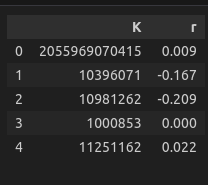
\includegraphics[height = 7cm]{img/graph_img/df8.png}
\end{frame} 

\begin{frame}{DataFrame para intervalos de 10 años}
    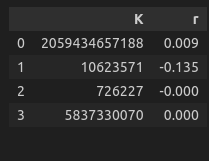
\includegraphics[height = 7cm]{img/graph_img/df10.png}
\end{frame} 

\section{Predicciones}
\begin{frame}{Predicción para intervalos de 5 años}
    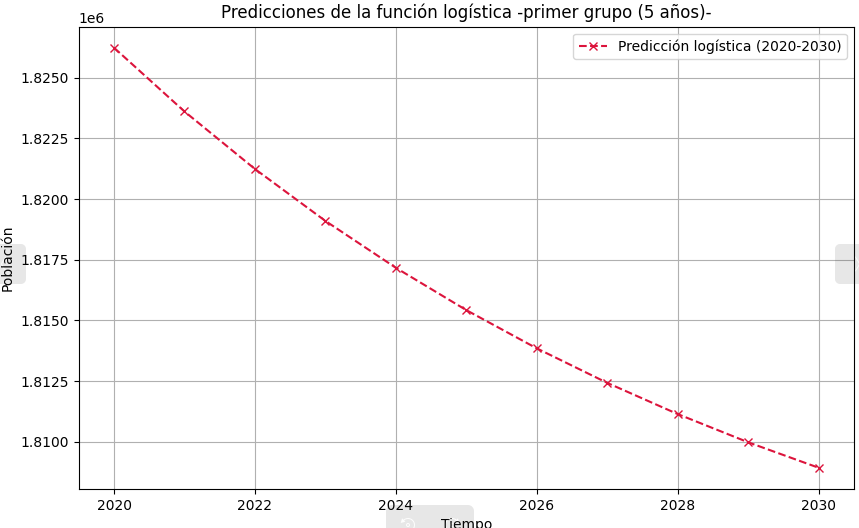
\includegraphics[height = 7cm]{img/graph_img/pred5.png}
\end{frame}

\begin{frame}{Predicción para intervalos de 8 años}
    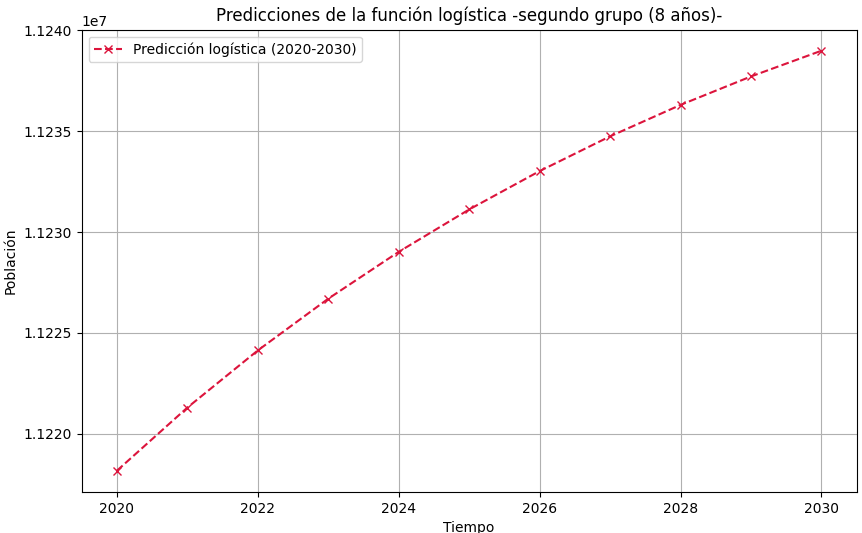
\includegraphics[height = 7cm]{img/graph_img/pred8.png}
\end{frame}

\begin{frame}{Predicción para intervalos de 10 años}
    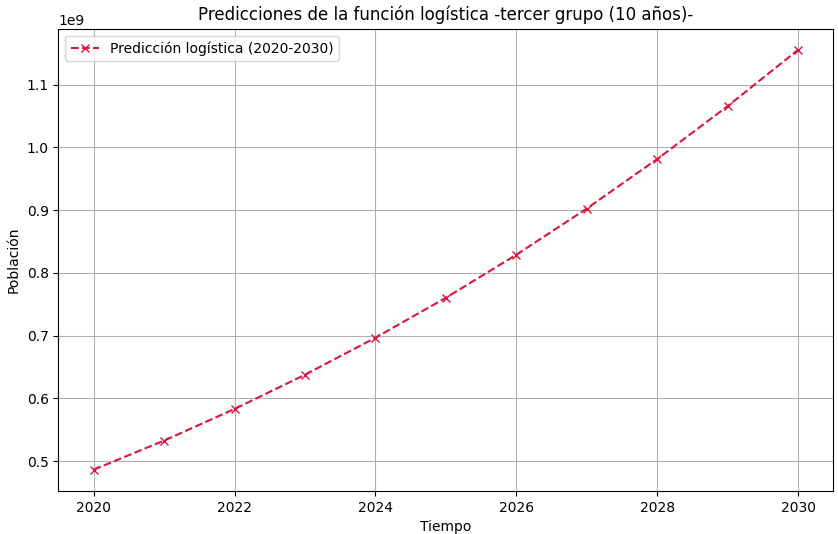
\includegraphics[height = 7cm]{img/graph_img/pred10.png}
\end{frame}

\section{End}
\begin{frame}
    \huge{\textbf{\textcolor{red}{The End}}}
    
\includegraphics[height = 7cm]{img/cuba3.jpeg}
\end{frame}

\end{document}